% \newpage

\begin{table}[t]
\centering
 \begin{tabular}{|c c l|} 
 \hline
 Software & LoC & Description \\  
 \hline\hline
 \multicolumn{3}{|c|}{\textbf{Network Middelware Programs}}\\
 \texttt{PRADS-0.2}             & 28,083      & IDS \\ 
 \texttt{snort-2.9.9}           & 336,082     & IDS \\ 
 \texttt{haproxy-1.7.9}         & 97,278      & Load Balancer \\ 
 \texttt{Openvpn-2.4.3}         & 120,018     & Open-source VPN \\
 \texttt{Squid-2.5.27}          & 291,433     & Web Cache\\
 \hline\hline
 \multicolumn{3}{|c|}{\textbf{Interet of Things Applications}}\\
 \texttt{midilib} & 3,042 & MIDI protocol library \\ 
 \texttt{libmodbus} & 5,567 & A serial communications protocol \\ 
 \texttt{Eclipse Paho-mqtt} & 30,406 & Open and standard messaging protocols for IoT \\ 
 \texttt{Eclipse Paho-mos} & 33,429 & An open source message broker \\ 
 \texttt{open62541} & 37,020 & An open source implementation of OPC UA \\ 
 \texttt{Eclipse Wakaama} & 20,480 & Open Mobile Alliance's LightWeight M2M protocol \\ 
 \texttt{AwaLWM2M} & 106,319 & OMA Lightweight M2M protocol \\ 
 \texttt{mbed TLS} & 77,727 & SSL Library mbed TLS \\ 
 \texttt{OpenSSL} & 516,007 & Toolkit for the Transport Layer Security \\ 
 \texttt{dnp3} & 141,555 & Distributed Network Protocol \\ 
 \texttt{libcoap} & 35,125 & C-Implementation of CoAP \\ 
 \texttt{OpENer} & 20,103 & An EtherNet/IP stack for I/O adapter devices \\ 
 \hline
 \end{tabular}
\caption {A list of protocol implementations covering complicated network
middleware and lightweight IoT applications. Note that LoC indicates the lines
of code.}
\label{tab:software}
\end{table}


\section{Extracting Finite State Machines pertaining to Target Protocol}
\label{sec:subsetting}

As is discussed in the section above, the ultimate goal of this research project
is to generate customized dialects for protocols. To achieve this, we must
design and develop a mechanism to extract state machines pertaining to
protocols. In this section, we first discuss the challenges of protocol
extraction. Then, we describe our preliminary exploration followed by our
proposed techniques.

\subsection{Challenges}

From the perspective of software development, one can implement a
set of protocols in different forms. For example, a software developer may make
two protocols sharing the same code fragments or implement them separately or
use different data structures to define the state machines pertaining to
corresponding protocols. As such, the challenges of this research task include
(1) identifying the common patterns of protocol implementations, (2) pinpointing
the states pertaining to a protocol and (3) tracking down the state machines
pertaining to target protocols. In the following session, we discuss how we
intend to tackle these challenges.

\subsection{Preliminary Exploration}
\label{sec:task1:obs}

\begin{wraptable}{r}{.38\textwidth}
\centering
\begin{tabular}{c}
\hspace{12pt}

\begin{lstlisting}  
typedef enum {
    WORK_ERROR,
    WORK_FINISHED_STOP,
    WORK_FINISHED_CONTINUE,
    WORK_MORE_A,
    WORK_MORE_B,
    WORK_MORE_C
} WORK_STATE;
\end{lstlisting}

\end{tabular}
\caption{An enumeration type containing 6 integral constants indicating all the states pertaining to a
transmission protocol in \texttt{OpenSSL}.}
\label{code:enum}
\end{wraptable} 

To tackle these challenges, we must understand how developers typically
implement protocols in software. In this project, we therefore plan to start
with studying the implementation of various protocols. As our preliminary
exploration, we manually investigated the protocol implementation in software
specified in Table~\ref{tab:software}. As we can observe in the table, the
software we studied covers not only complicated network middleware like
\texttt{HAProxy} and \texttt{OpenVPN} but also lightweight IoT applications such
as \texttt{midilib} and \texttt{AwaLWM2M}. In the following, we summarize the
key observations obtained from this preliminary manual study.

Based on our manual study across all the software in Table~\ref{tab:software},
we first observe that a stateful protocol is typically implemented either in a
loop or a call back function. For example, Table~\ref{code:midilib} shows a
transmission protocol that is implemented in an infinite loop~\footnote{We consider 
a loop not iterating a specified number of times as an infinite loop.}. 
We believe that
this observation can be generalized, and an infinite loop or a call back can be
used for identifying a protocol implementation. This is due to the fact that a
stateful protocol is a finite state machine that needs to retain session
information and keep alive during program execution, and the best practice of
implementing such a protocol is through an infinite loop or a call back
function.

In addition to using a loop or a call back to implement a stateful protocol, we
observe that software developers typically utilize the enumeration data type
(\texttt{enum}) to define the states pertaining to a state machine. As is shown
in Table~\ref{code:enum}, for example, \texttt{WORK\_STATE} is an enumeration
type, which consists of 6 integral constants indicating all the states
pertaining to a transmission protocol in \texttt{OpenSSL}.

From our manual investigation,  we also observed that enumeration type is not
always used for the definition of protocol states nor the only data type that
implements states pertaining to a protocol. However, we believe it can be
potentially used to facilitate the identification of variables that implement
the states of a protocol. In the following section, we will discuss how we
intend to do so by taking this observation.

\begin{wraptable}{r}{.38\textwidth}
\centering
\begin{tabular}{c}
\hspace{12pt}

\begin{lstlisting}  
/* midifile.c */
bool midiReadGetNextMessage(const MIDI_FILE *_pMF, int iTrack, MIDI_MSG *pMsg) {
	if ((pMsg->iType & 0xf0) != 0xf0)
		...
}

/* m2rtttl.c */
MIDI_MSG msg; // MIDI_MSG is a struct type
... 
while(midiReadGetNextMessage(mf, i, &msg)) {
	...
	if (iCurrPlayingNote==msg.MsgData.NoteOff.iNote) {
		...
		iCurrPlayingNote = -1;
		...
	}
	...
}
\end{lstlisting}

\end{tabular}
\caption{The code fragments indicating the implementation of midi protocol.}
\label{code:midilib}
\end{wraptable} 

Last but not least, we observe software developers tend to use composite data
type to define the data packets exchanged between communication entities.
Typically, this kind of data structures is involved in bitwise operations and
tied to function calls pertaining to message read and write. For example, the
\texttt{midi} protocol defines data packet \texttt{msg} in struct
\texttt{MIDI\_MSG}. As is shown in Table~\ref{code:midilib}, software developers
tie it to message read function \texttt{midiReadGetNextMessage} and utilize
bitwise operations (see \texttt{lines 3}) to examine the values in this data
structure. In this project, we plan to leverage this observation to facilitate
the identification of the data structure pertaining to the data packets of the
target protocols. Though it might introduce some false positives or false
negatives, we believe this observation is relatively reliable for data structure
identification for the following reason. In most protocols, the information must
be packed into the data block without leaving any unused bits between the
fields. To make the best use of a data packet, the best practice is to make
extensive use of bitwise and shift operators to take the information values and
pack them into the payload being transmitted. In the following, we will further
discuss how we intend to utilize the key observations above to perform protocol
extraction or in other words the state machines pertaining to protocols residing
in the target software.

\subsection{Proposed Techniques}

Following the observations above, we will design and develop a series of
technical approaches to (1) identify the code fragments representing protocol
implementation, (2) pinpoint the variables that
implement the states of protocols, and (3) track down the state transitions and
thus construct the finite state machines pertaining to the protocols in target
software. In addition, we will explore, design and develop technical approaches
to refine the state machines, making sure the state machines extracted truly
represent that specified in a target protocol. In the following section, we
describe and discuss how we plan to design and develop these techniques in more
details.

\subsubsection{Research Task 1: Identifying Code Fragments Pertaining to
Protocol Implementation}
\label{subsec:rt1}

As is described above, the protocol implementation is typically associated with
an infinite loop or a call back function. In this project, we intend to use this
pattern to narrow down the implementation of a protocol in source code. In
particular, we plan to perform an exhaustive search on the code base of target
software, extract all the infinite loop and call back functions and treat these
as the candidates of protocol implementation. As is mentioned above, this
candidate set however may contain implementation not relevant to protocols.
Therefore, we will further introduce some heuristics to reduce false positives
and negatives introduced by this trivial approach.

Intuition suggests that the implementation of a stateful protocol must contain
the state variables, and the transitions between states must depend upon the
data packets transmitted. As a result, going beyond simply identifying infinite
loops and call back functions, our technique will examine if the state variable
is included in the candidate code fragments. In addition, we augment our
protocol identification technique with the ability to examine if state
transitions are engaged in the loops or call back functions.

Technically, it is trivial to check whether a state variable is involved in a
code fragment as along as one can correctly pinpoint the variable that
implements the state of a protocol. In this proposal, Section~\ref{subsec:rt2}
specifies how we plan to identify state variables using the observation
described above. With regard to the approach to examine state transitions in a
loop or call back function, we intend to perform reachability analysis within
the loop or call backs. In particular, we will perform liveness analysis on a
state variable in two consecutive iterations\footnote{It should be noted that we
treat a call to the callback function as one iteration.}. Then, we conduct a
control dependence analysis so that we can examine whether the definition 
of that state variable
depends on its use. The design principle behind this approach is that --
in a loop or a call back -- 
control dependence and liveness analysis can identify if there
exists a state transition from one to another.

We illustrate this approach by taking midi protocol for example. As is shown in
Table~\ref{code:midilib},  the midi protocol is implemented in a loop where
\texttt{iCurrPlayingNote} indicates the state variable. By performing liveness
analysis in two consecutive iterations, we can easily pinpoint that 
the definition of variable \texttt{iCurrPlayingNote} in
\texttt{line 14} depends on \texttt{line 12}.
This indicates the state variable must be changed to
\texttt{-1} if the current state is \texttt{msg.MsgData.NoteOff.iNote} or in
other words there exists a state transition from
\texttt{msg.MsgData.NoteOff.iNote} to state \texttt{-1}. From the code fragment
shown in Table~\ref{code:midilib}, we can also discover  the transition
identified is dependent upon the message indicated in \texttt{line 8}.


% https://github.com/MarquisdeGeek/midilib/blob/master/src/m2rtttl.c#L193	  


\subsubsection{Research Task 2: Pinpointing the Variables Implementing the
States of Protocols}
\label{subsec:rt2}

As is mentioned and showcased in Section~\ref{sec:task1:obs}, enumeration type
is a critical indicator for identifying variables pertaining to protocol states.
However, it is not always the case whether variables in that type serves as the
implementation of protocol states. As a result, we must have a mechanism to
distinguish variables that truly represent the states of a protocol. In this
project, we intend to achieve this by performing a simple but effective
verification. In particular, we will examine each variable in enumeration type
and verify if that variable is present in the code fragment representing the
implementation of a stateful protocol. This is simply because the implementation
of a stateful protocol must contain state transitions.

Considering enumeration is not the only data type that can be used for
implementing protocol states, the project will further explore other indicators
that could  potentially facilitate the identification of state variables. Going
beyond variables in enumeration type, for example, we may take into consideration
other variables introduced to the code fragments pertaining to protocols. More
specifically, we could focus on those integer variables, the values of which
are discrete and bounded in a certain range, for the reason that a state machine
pertaining to a stateful protocol must have a finite number of states. In
addition, we will ensure the scope of those variables are not limited within 
one loop iteration or one call back invocation. This is because the state machine must stay
live across iterations.
In this project, we plan to perform value set analysis
and live variable analysis to  to determine the value set for variables as well
as their liveness respectively.

To illustrate this solution, we take for example the code fragment shown in
Table~\ref{code:midilib}. Variable \texttt{iCurrPlayingNote} is in an integer
type. By performing a flow, context and path sensitive value set analysis, we
can figure out its value set includes \texttt{-1} and
\texttt{msg.MsgData.NoteOn.iNote} where \texttt{msg.MsgData.NoteOn.iNote} is
another variable with a constant value. Using live variable analysis, we can
also pinpoint the liveness of variable \texttt{iCurrPlayingNote} is beyond one iteration 
of the loop indicated in Table~\ref{code:midilib}, and thus treat it as
the variable potentially implementing the protocol state. As part of this
project, we will evaluate the effectiveness of this proposed technique using
various protocols and their implementations.


% -----------------------------------------------------------------------------

\begin{figure*}[t]
\centering
\subfloat[Invalide state machines.]{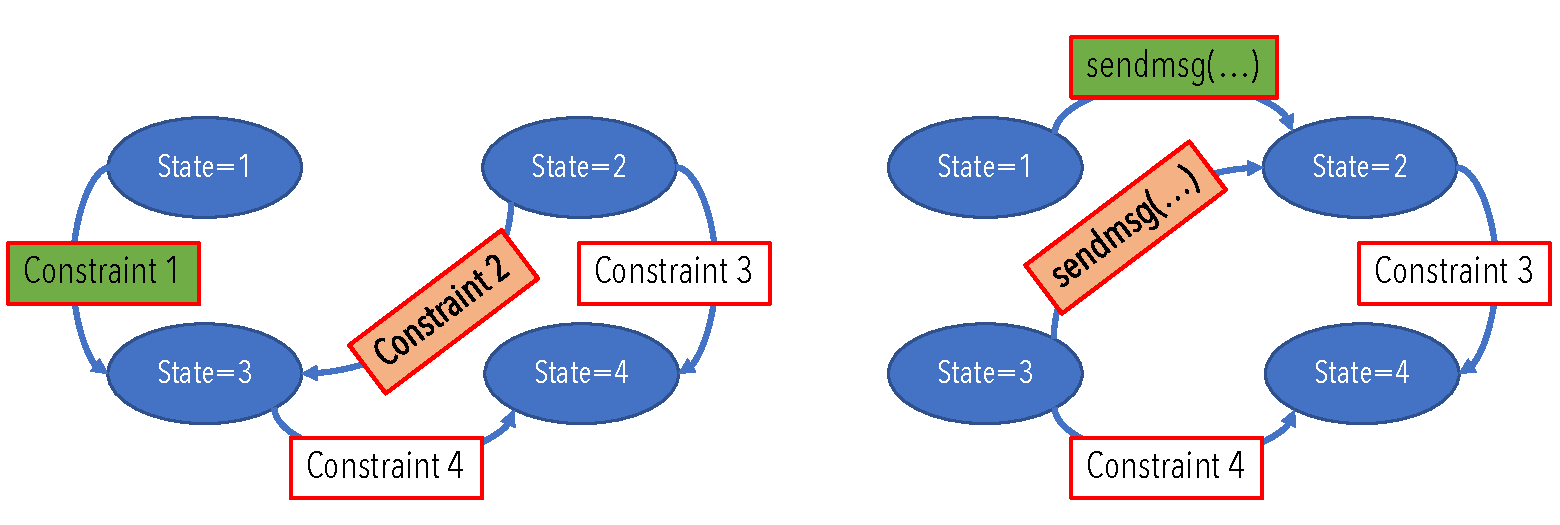
\includegraphics[width=0.47\linewidth]{figure/fsm1}\label{fig:invalid}} 
\hspace{0.05\textwidth}
\subfloat[Legitimate state machines.]{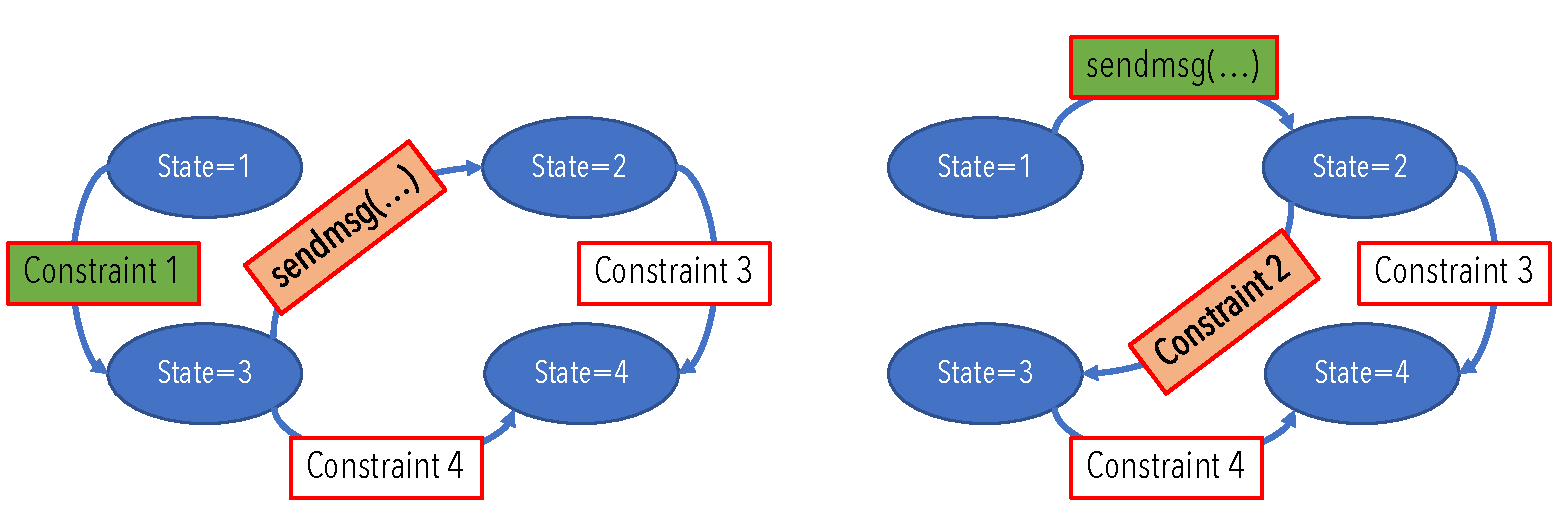
\includegraphics[width=0.47\linewidth]{figure/fsm2}\label{fig:valid}}
% \vspace{-0.1in}
\caption{Finite state machines decoupled from that indicated in Figure~\ref{fig:fsm0}.} 
\label{fig:fsm} 
\end{figure*} 

% -----------------------------------------------------------------------------

\subsubsection{Research Task 3: Constructing Finite State Machine}
\label{subsec:rt3}

With the protocol implementation and state variables identified in source code,
we now discuss how we intend to construct the state machines pertaining to the
target protocol. Since a state machine consists of not only a finite set of
states but also a series of transition conditions, we must have a mechanism to
extract the condition pertaining to each transition. In this project, we plan to
achieve this goal by performing a partial symbolic execution. To be specific, we
will first perform a breadth first search within the code fragment pertaining to
protocol implementation. With this search, we aim to identify the path tied to
each state transition. Since the constraints along a path indicates the
conditions of a possible state transition, for each path identified, we will
further perform a partial symbolic execution and record the constraint along
that path.

With the design above, we can build a transition table, where each entry carries
a pair of states as well as their transition condition. It is not difficult to
notice that we can easily construct a finite state machine using this transition
table. However, this might provide us with a state machine not truly
representing the protocol specification simply because a software developer
might implement two different protocols by sharing the same code fragment (e.g.,
the implementation of \texttt{OpenVPN}~\citep{openvpn-github}). To address this
issue, we intend to augment our protocol extraction technique with  an ability
to  decouple  state machines.

\begin{wrapfigure}{r}{0.3\textwidth}
  \centering
  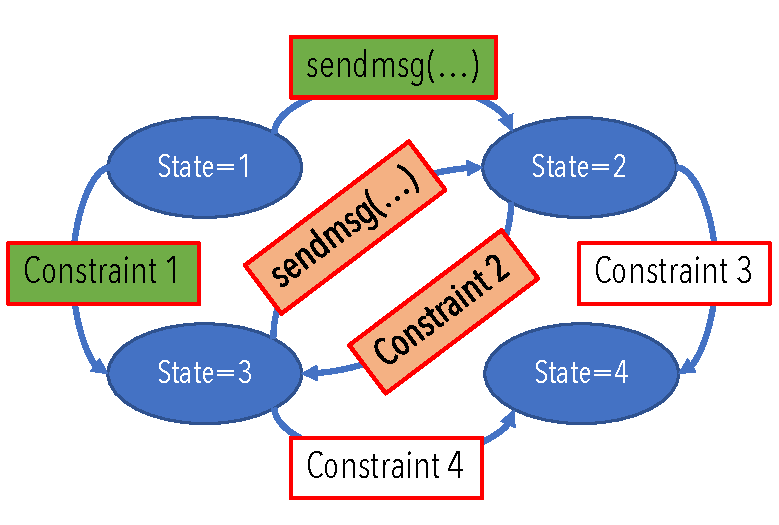
\includegraphics[width=0.3\textwidth]{figure/fsm0}
  \caption{A finite state machine carrying two independent ones.}
  \label{fig:fsm0}
\end{wrapfigure}

A finite state machine changes from one state to another in response to some
external inputs. Intuition suggests these inputs cannot be generated from the
state machine itself. Therefore, if a state machine receives a packet from
itself, it implies that the state machine extracted does not represent the
protocol specification and we must perform a state machine partition. To do it,
we plan to attach message write operations to corresponding edges on a state
machine, and then pair each of these operations with the message read. With this
design, we can decouple state machines accordingly. To illustrate this, we take
for example the state machine shown in Figure~\ref{fig:fsm0}. Assume the
rectangles in the same color indicate message read and write operations paired
together. Following the aforementioned criteria -- that a state machine cannot
receive a message sent by itself -- we can separate the state machine into four
ones as is demonstrated in Figure~\ref{fig:fsm}. From this figure, we can
observe none of these state machines decoupled involves receiving a message sent
by itself. In addition, we can observe two state machines are invalid and can be
easily eliminated because none of them includes a path along which one can
traverse all the states (see Figure~\ref{fig:invalid}). For the legitimate state
machines shown in Figure~\ref{fig:valid}, we will deem them as 
the potential finite state
machines pertaining to the target protocol.

In this project, we will explore various program analysis approaches to
implement the proposed techniques. To pair inbound and outbound messages, for
example, we can perform value set analysis against the outgoing messages prior
to its attachment to message sending, and then match that value set with the
constraints on the edges. With regard to retrieving transition conditions, we
will perform pointer analysis and build an interprocedural control flow graph
pertaining to the code fragment of the interest. Then, we will perform the
aforementioned breath first search on the graph and identify the paths
pertaining to state transitions. By modifying \texttt{KLEE} compatible with the
latest version of \texttt{LLVM}, we intend to develop a partial symbolic
execution to perform path-specific constraint extraction. Last but not least, we
will also check the constraints tied to state transitions by running constraint
solvers (\eg, \texttt{Z3} or \texttt{SMT}). This will allow us to examine the
validity of the conditions tied to transitions.

 % https://en.wikipedia.org/wiki/Finite-state_machine